\section{Business Process Management Tools}
% Business Process Management (BPM) is a methodology that involves designing, controlling, and analysing business processes to support organisations \cite{bpmdefinition}. 
% BPM's stages is defined differently depending on references \cite{bpmlifecycles, bpmlifecycles2, bpmlifecycles3}; however, it generally consists of at least four stages: i) analysing; ii) modeling; iii) implementing; iv) executing.
% As for BPM tools, they are software solutions that support organisations in all stages of BPM with little to no coding knowledge. As a consequence, BPM tools are widely used in various industries.
Business Process Management (BPM) is a concept that assist business analysts in planning, monitoring and analysing business processes to support organisations \cite{bpmdefinition}. BPM could be separated into stages depending on references being used \cite{bpmlifecycles, bpmlifecycles3, bpmlifecycles2}, but generally, it consists of four different stages: i) analysing; ii) modelling; iii) implementing; iv) execution. Software that makes use of this concept in assisting business analysts model processes with little to no coding knowledge is known as BPM tools.

One of the advantages of using BPM tools is the orchestration between systems, humans, and workflows \cite{bpmstrength}. This improves the overall efficiency of business processes in organisations \cite{bpmbenefits}. BPM tools use checklists that are integrated as part of a workflow to efficiently coordinate humans and workflows. For example, Bizagi \cite{bizagi}, one of the famous BPM tools, can construct checklists or forms within its automated workflows and connect the checklists to the following processes using the shared database technique. Nintex \cite{nintext} is another widely used BPM tool that also adopts the idea of checklist and implements it in their environment. This provides a variety of options for workflow users to interact with the workflows in the system.


\section{WorkflowFM: A logic-based framework for formal process specification and composition}
\label{background:workflowfm}

% WorkflowFM \cite{papapanagiotou2017workflowfm} is a logic-based BPM tool developed by researchers from the University of Edinburgh. Being a logic-based framework means all the inputs, outputs, and processes follow the validation defined by the framework.
% Each process is validated by WorkflowFM to ensure that it is logically valid and functional as a workflow.
As a logic-based BPM tool, WorkflowFM differs from other frameworks in that it requires inputs and outputs in each process to match when connected to other processes, as opposed to most BPM tools which accept any viable XML format when creating a workflow.
% Additionally, WorkflowFM requires defining data models for each input and output
% only require a XML pattern to create a workflow as XML is the standardised format for BPM tools.
% unlike various BPM tools which follows the XML Process Definition Language (XPDL), the standard format for interchanging process definitions between different BPM tools \cite{xmlpdl}.

WorkflowFM's system architecture, as shown in Figure \ref{fig:workflowfm-system}, includes two main components: modelling and execution. Modelling is the part that allows workflow users to create workflows and validates workflows by the reasoner. On the other hand, execution is the component that operates workflows that has been deployed. Execution contains the execution engine, the simulation engine, the checklist generation, and the dashboard. The checklist generation connects with the execution engine as an extension to generate checklists and allow people to perform tasks for executing workflow processes.
% The execution engine and the simulation engine are integrated with each other and directly connect to the dashboard to visualise deployed workflows. Furthermore, the checklist generation connects with the execution engine as an extension to generate checklists and allow people to perform tasks for workflows.
% Unlike Bizagi or Nintex, WorkflowFM is a logic-based framework which 

\begin{figure}
    \centering
    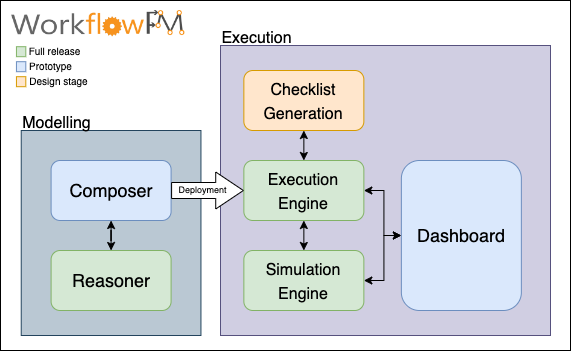
\includegraphics[width=0.7\textwidth]{overleaf/images/workflowfm-system.png}
    \caption{WorkflowFM's System Architecture}
    \label{fig:workflowfm-system}
\end{figure}

As of now, WorkflowFM has been used in the healthcare and manufacturing domains. With the expanding usage of the framework, the checklist generation becomes more desirable for people in the industries. However, checklist generation is still at the design stage and has not been implemented. That is why this project focuses on implementing a prototype of the checklist generation.

% As of now, WorkflowFM has been used in the healthcare domain \cite{papapanagiotou2014formal} and expanding to the manufacturing domain. With in increasing of ..., this is why a checklist generation tool is needed in WorkflowFM.

\section{WorkflowFM's Process Input and Output}
\label{background:input_output}

The JSON format \cite{json} is used in WorkflowFM to construct processes. The JSON includes several fields that are used in different parts of the system, which can be seen in Figure \ref{fig:workflowfm_json}. However, the name, input and output of each process are the only requirements to generate a resource-based checklist template.
% Each model consists of \verb!type!, \verb!name!, and \verb!args!. There are only three types in \verb!type!: \verb!var!, \verb!plus!, and \verb!times!. 

\begin{figure}[ht!]
    \centering
    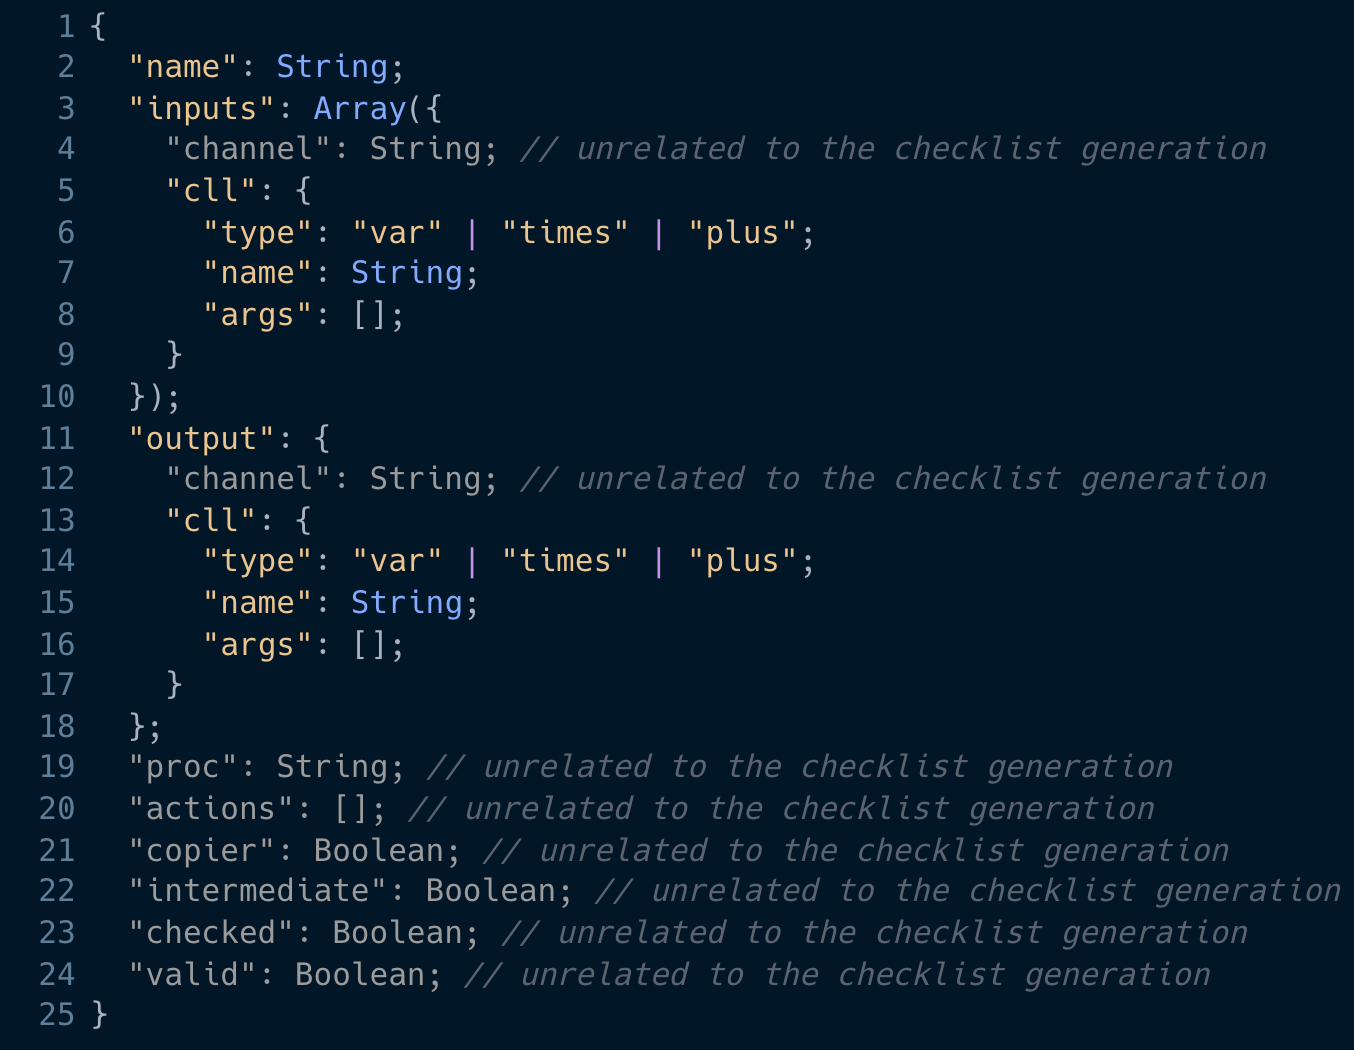
\includegraphics[width=0.75\textwidth]{overleaf/images/workflowfm_json.png}
    \caption{WorkflowFM's Process JSON}
    \label{fig:workflowfm_json}
\end{figure}


% Each input and output node can only be in one of the three types including \verb!var!, \verb!times!, and \verb!plus!.
% A \verb!var! node is a terminal node. That means a \verb!var! node must have no child. Being a \verb!var! node indicates that that specific node is a data model that the process can refer to.
% On the other hand, \verb!times! and \verb!plus! nodes are not data models on its own and must contain child nodes inside it. The child nodes can either be one of the three types recursively, but at terminal nodes, they must be the \verb!var! type.
% \verb!times! and \verb!plus! nodes are different on how they combine the children. \verb!times! merges all the children together as one large data model, while \verb!plus! only selects one of its children to be the data model representing that node.

% All child nodes under \verb!times! are required to exist as the data model representing that node, while only one of the children under \verb!plus! is the representative data model. 

% but they must contain nodes as their children. The difference between \verb!times! and \verb!plus! is all child nodes in a \verb!times! node are compulsory inputs or outputs, while a \verb!plus! node needs only one of the child nodes to be an input or output.

% A process contains nodes from both input and output sides. A node is a representation between three things: a data model, a times operator, and a plus operator. A data model will be referred as the \verb!var! type. A times operator and a plus operator will be referred as \verb!times! and \verb!plus! accordingly. Both \verb!times! and \verb!plus! nodes must contain children since they are not data models. Furthermore, their children can either be \verb!var!, \verb!times!, and \verb!plus!. However, if a child node is either \verb!times! or \verb!plus!, it needs to recursively continue having children. A \verb!var! child, however, contains no children and acts as a terminal node. \verb!times! and \verb!plus! are different on how they operate. \verb!times! combines the children together as one large data model, while \verb!plus! only selects one of its children to be the data model representing that node.

The input and output of a process are represented as nodes. A node can either be an atomic entity (\verb!var!) \cite{entity} or an operator (\verb!times! or \verb!plus!).
An atomic entity represents an entity in the system's database.
An operation which combines multiple nodes is called a times operator, while which selects an entity between a group of nodes is called a plus operator.
Combining both entities and operators would form into a tree of nodes, which a leaf node of this tree must be an entity.

For example, in Figure \ref{fig:process_flows} | which has the JSON format provided in Appendix \ref{appendix:fig:example_json}, this is a payment process that receives \verb!orders! and \verb!payment_method! as the input and returns \verb!order_receipt! and either \verb!credit_card_receipt! or \verb!change! as the output depending on what \verb!payment_method! coming in.
All five of them are terminal nodes and data models of this process. On the input part, both \verb!orders! and \verb!payment_method! are connected to a \verb!times! node indicating that both data models are compulsory. Meanwhile, \verb!credit_card_receipt! and \verb!change! are connected to a \verb!plus! node indicating either one between them can be selected as the representing data model; however, not both. On top of that, the \verb!plus! node is connected to a \verb!times! node along with \verb!order_receipt! indicating both of them are compulsory.

Ultimately, the input of this payment process is ``\verb!orders! and \verb!payment_method!"; and the output of this payment process is either ``\verb!order_receipt! and \verb!change!" or ``\verb!order_receipt! and \verb!credit_card_receipt!".

% the input node is a \verb!plus! and contains two children: \verb!input_var_node_1! and \verb!input_times_node!. Moreover, one of the children is a \verb!times! and contains two children: \verb!input_var_node_2! and \verb!input_var_node_3!. Ultimately, the input of this process can be either:

% \begin{itemize}
%     \item \verb!input_var_node_1! \vspace{-8px}
%     \item (\verb!input_var_node_2!, \verb!input_var_node_3!)
% \end{itemize}

% The output of the process is less complex in comparison to the input.
% The output node is a \verb!times! and has only two \verb!var! children. This makes (\verb!output_var_node_1!, \verb!output_var_node_2!) as the output of this process.

% That means either \verb!input_var_node_1! or \verb!input_var_node_2! can be the input data model of the process. Meanwhile, the output node is \verb!times! and also contains two children. In contrast to \verb!plus!, \verb!output_var_node_1! and \verb!output_var_node_2! are the output data models of the process.

\begin{figure}[ht!]
    \centering
    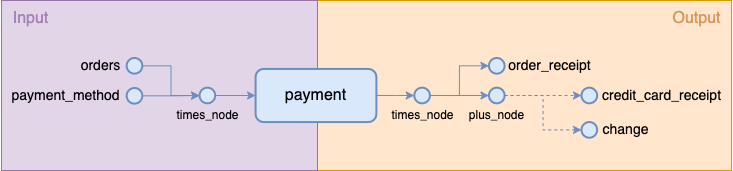
\includegraphics[width=\textwidth]{overleaf/images/process_flows.png}
    \caption{Example Process}
    \label{fig:process_flows}
\end{figure}

\section{Generation of structured checklists from formal \\resource-based workflow models}
\label{background:chens_design}
% This is an MSc project from the previous year written by Yefei Chen \cite{checklistdesign}. Chen has designed the user interface for WorkflowFM's checklist generation tool as well as solved some of the theoretical challenges in the design, such as function-flow chart and data model design. Chen's design consists of six features: i) main page; ii) canvas; iii) edit checklist dependencies; iv) process checklist; v) finished checklist; vi) design of checklist. In the end, the system usability scale questionnaire (SUS) score was mediocre, with a score of 56.5. However, Chen discussed the design weaknesses and provided an analysis of them. Consequently, the results are extremely important since we could continue improving the design based on the analysis.

A design of a resource-based checklist generator has been proposed in Yefie Chen's MSc dissertation \cite{checklistdesign}. Chen designed this tool based on the concept of WorkflowFM that contains all the data models of the workflow processes in the system. The design utilises the benefits of WorkflowFM and gives users the ability to develop checklists that link to data models of workflow processes via checklist dependencies.
The design consists of four user interfaces with functionalities on each screen as follow:

\begin{itemize}
    \item \textbf{Main Page} is the landing screen of the checklist generator. It can be divided into three sections: \verb!Start A Checklist!, \verb!In Progress!, and \verb!Finished!. The \verb!Start A Checklist! section will bring the user to Canvas screen to create a template. The \verb!In Progress! section is the section that contains all the checklists that has already been started, but not yet finished. And lastly, the \verb!Finished! section contains all the finished checklists.
    \item \textbf{Canvas} is the building templates screen. It allows users to custom the title, question names, types, and other things in checklists.
    \item \textbf{Edit Checklist Dependencies} is the screen to manage dependencies in a template. Once a template has been created in Canvas, the designer sometimes needs to adjust dependencies between the input and output. That is to allow the system to create connections between components.
    \item \textbf{Process Checklist} is the screen of a finished template. It displays the information according to the designed template in Canvas. A finished template, or checklist, in this screen will be used to perform tasks for workflow processes in WorkflowFM.
\end{itemize}

